\documentclass[12pt]{article}
\usepackage[cm]{fullpage}
\usepackage{listings}
\usepackage{color}
\usepackage{xcolor}
\usepackage{textpos}
\usepackage{amssymb,latexsym}
\usepackage{amsmath}
\usepackage{xltxtra,xunicode,xgreek}
\usepackage[colorlinks=true, linkcolor = blue, citecolor=blue]{hyperref}
\usepackage[ddmmyyyy]{datetime}
\usepackage{float}
\usepackage{textcomp}
\usepackage{url} 
\usepackage{turnstile}
\usepackage{xcolor,colortbl}
\usepackage{mathtools}
\usepackage{minted}

\definecolor{gray}{gray}{0.89}
\definecolor{ablack}{HTML}{25383C}
\setmainfont[Mapping=tex-text]{CMU Concrete}
\setmonofont{Courier New}
\newcommand{\tab}{\hspace*{2em}}
\newcommand{\rom}[1]{\uppercase\expandafter{\romannumeral #1\relax}}
\setlength{\parindent}{0pt}
\usemintedstyle{tango}

\newcommand{\Llama}{\textsf{Llama }}

\usepackage{caption}
\DeclareCaptionFont{white}{\color{white}}
\DeclareCaptionFormat{listing}{\colorbox{gray}{\parbox{\textwidth}{#1#2#3}}}
\captionsetup[lstlisting]{format=listing,labelfont=white,textfont=white}
%\renewcommand\listingscaption{Κώδικας}
\renewcommand{\arraystretch}{1.5}


\begin{document}
\begin{titlepage}
\begin{center}


\includegraphics[scale=0.3]{pyrforos.jpg}\\
ΕΘΝΙΚΟ ΜΕΤΣΟΒΙΟ ΠΟΛΥΤΕΧΝΕΙΟ \\
ΣΧΟΛΗ ΗΛΕΚΤΡΟΛΟΓΩΝ ΜΗΧΑΝΙΚΩΝ KΑΙ ΜΗΧΑΝΙΚΩΝ ΥΠΟΛΟΓΙΣΤΩΝ \\ 
\vspace{0.5em}

\medskip 

\def\doubleline{

    \vspace{0.1em}
    \line(1,0){530}\

    \vspace{-1.5em}
    \line(1,0){530}

}
\doubleline
\vspace{1.3em}

{\large \textbf{Μεταγλωττιστές}\\
 \medskip
8ο εξάμηνο, Ακαδημαϊκή περίοδος 2012 \\ \bigskip \medskip}

\vspace{1.5em}
{\LARGE \textbf{Υλοποίηση της γλώσσας \Llama\\}}
\vspace{1cm}
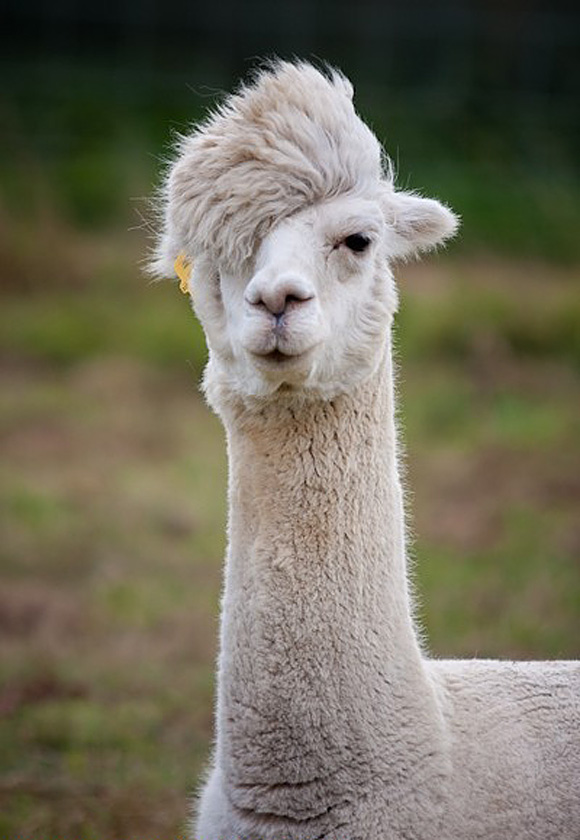
\includegraphics[scale=0.4]{llama.jpg}\\
\vfill
\begin{tabular}{l l}
Kωνσταντίνος Αθανασίου & 03108132\\
Νίκος Γιανναράκης & 03108054 \\
Ζωή Παρασκευοπούλου & 03108152 \\
\end{tabular}\\
\bigskip
\today
\end{center}
\end{titlepage}
\tableofcontents

\pagebreak

\section{Εισαγωγή}
H \Llama είναι μια γλώσσα η οποία συνδυάζει στοιχεία συναρτησιακού και προστακτικού προγραμματισμού και συντακτικά μοιάζει αρκετά με τη γλώσσα Caml. Η εργασία έχει υλοποιηθεί στη γλώσσα OCaml. Αναλυτικά οι προδιαγραφές τις γλώσσας βρίσκονται \href{http://courses.softlab.ntua.gr/compilers/2012a/llama2012.pdf}{εδώ}.
\section{Χρήση}
Για τη μεταγλώττιση του μεταγλωττιστή χρειάζονται τα παρακάτω:
\begin{itemize}
\item \href{http://ocaml.org/install.html}{OCaml 4.0.0} ή νεότερη έκδοση
\item \href{http://ocamlgraph.lri.fr}{Ocamlgraph} ή μέσω \href{http://opam.ocaml.org/pkg/ocamlgraph/}{OPAM}
\item \href{http://pauillac.inria.fr/~ddr/camlp5/}{CamlP5} ή μέσω \href{http://opam.ocaml.org/pkg/camlp5}{CamlP5}
\end{itemize}

Η διαδικασία μεταγλώττισης είναι η παρακάτω:
\begin{itemize}
\item[\$] make depend
\item[\$] make
\end{itemize}

Εναλλακτικά μπορεί εξαχθεί native εκτελέσιμο εκτελώντας τα παρακάτω

\begin{itemize}
\item[\$] make depend
\item[\$] make Llama.opt
\end{itemize}

Προαιρετικά, μπορεί να εξαχθεί το API του compiler σε αρχεία html μέσω της εντολής:
\begin{itemize}
\item[\$] make doc
\end{itemize}

Για την μεταγλώττιση ενός αρχείου πηγαίου κώδικα \Llama απαιτούνται τα παρακάτω βήματα:

\begin{itemize}
\item[\$] ./Llama file.lla
\end{itemize}

ή

\begin{itemize}
\item[\$] ./Llama.opt file.lla
\end{itemize}

Επιπλέον παρέχονται οι εξής επιλογές:

\begin{table}[htbp]
\centering
\begin{tabular}{|l|l|}
\hline
   \rowcolor{ablack}
    \textcolor{white}{Option} & \textcolor{white}{Description} \\ \hline
    
    \rowcolor{gray}
    -O & Εκτέλεση βελτιστοποιήσεων \\ 
    
    -i & Παραγωγή ενδιάμεσου κώδικα \\ 
    
     \rowcolor{gray}
    -g & Παραγωγή γράφου ελέγχου ροής σε .dot αρχείο \\
    
    -help & Προβολή διαθέσιμων επιλογών \\ 
    
\hline
\end{tabular}
\caption{Command-line options}
\end{table}

Για την εκτέλεση του μεταγλωττισμένου αρχείου $file.asm$ χρειάζονται τα παρακάτω:
\begin{itemize}
\item \href{http://www.dosbox.com/}{dosbox}
\item masm
\item Η βιβλιοθήκη χρόνου εκτέλεσης llama.lib που περιέχεται στην υλοποίηση μας
\end{itemize}

Η συμβολομετάφραση μπορεί να γίνει εκτελώντας την παρακάτω εντολή στο περιβάλλον του dosbox:
\begin{itemize}
\item[>] ml.exe file.asm llama.lib
\end{itemize} 
οπότε και παράγεται το εκτελέσιμο αρχείο $file.exe$.
Το εκτελέσιμο που παράγεται έχει μέγεθος stack $32KB$ το οποίο μπορεί να τροποποιηθεί μέσω κατάλληλου ορίσματος στον Microsoft Linker.
%
%Compiler project for NTUA compilers course. 
%
%The language scpecification can be found [here](http://courses.softlab.ntua.gr/compilers/2012a/llama2012.pdf) in greek.
%
%
%Llama is a functional programing language, inspired from Caml, featuring:
%
%* Type Inference 
%* High order functions
%* User defined data types
%* Imperative features: destructive arrays, mutable variables, while and for loops
%
%
%**Dependencies:**
%
%* [*OCaml*](http://ocaml.org/install.html) version 4.0.0 or newer
%* [*OCamlgraph*](http://ocamlgraph.lri.fr) or via OPAM [here](http://opam.ocaml.org/pkg/ocamlgraph/1.8.3/)
%* [*CamlP5*](http://pauillac.inria.fr/~ddr/camlp5/) or via OPAM [here](http://opam.ocaml.org/pkg/camlp5/6.11/)
%
%**To compile:**
%
%    $ make .depend
%    $ make
%    
%Optionaly, you can create the documentation files: 
%    
%    $ make doc
%
%
%**To run:**
%
%    $ ./Llama file.lla
%    $ dosbox
%    $ ml.exe file.asm llama.lib
%
%
%You can type 
%	
%	./llama --help


\section{Υλοποίηση}
Στην ενότητα αυτή θα παρουσιάσουμε συνοπτικά κάποια βασικά στοιχεία της υλοποίησης.
\subsection{Συντακτικός και Γραμματικός Αναλυτής}
Για τον συντακτικό αναλυτή χρησιμοποιήθηκε το εργαλείο \href{http://courses.softlab.ntua.gr/compilers/2012a/ocamlyacc-tutorial.pdf}{Ocamllex} και για τον γραμματικό     αναλυτή το εργαλείο \href{http://courses.softlab.ntua.gr/compilers/2012a/ocamlyacc-tutorial.pdf}{Ocamlyacc}.


\subsection{Σημασιολογική Ανάλυση}
Ο σημασιολογικός αναλυτής της \Llama εισάγει τις απαραίτητες πληροφορίες στο symbol table και ελέγχει κατά πόσο οι μεταβλητές του προγράμματος χρησιμοποιούνται ορθά, για παράδειγμα αν έχουν δηλωθεί πριν τη χρήση. Επιπλέον μέσω του αλγορίθμου εξαγωγής τύπων, κάνει έλεγχο τύπων και ανακατασκευάζει τους τύπους που δεν έχουν δηλωθεί από τον προγραμματιστή με κάποιο type annotation.


\subsubsection{Εξαγωγή Τύπων}
Η εξαγωγή τύπων βασίζεται στην παραγωγή περιορισμών κατά τη διάσχιση του ast, υπό τη μορφή εξισώσεων τύπων, και κάθε άγνωστος τύπος αναπαριστάται από μια μοναδική μεταβλητή τύπου. Στο τέλος της διάσχισης, καλείται η συνάρτηση unify, η οποία λύνοντας τους περιορισμούς αναθέτει σε κάθε μεταβλητή τύπου έναν γνωστό τύπο. Σε περίπτωση που οι περιορισμοί δεν είναι επιλύσιμοι επιστρέφεται μήνυμα λάθους, το οποίο επισημαίνει τους δύο τύπους που δεν μπορούν να ενοποιηθούν.


Στην γλώσσα \Llama οι τελεστές σύγκρισης υποστηρίζονται μόνο για τους τύπους int, float και char. Προκειμένου να ελέγξουμε στατικά αυτόν τον περιορισμό δημιουργούμε έναν καινούριο τύπο ord που αναπαριστά τους τύπους που υποστηρίζουν τελεστές διάταξης. Έτσι προκύπτει ο παρακάτω κανόνας τυποποίησης:

$$\frac{\Gamma  \vdash e_1 : ord \;\;\;\; \Gamma  \vdash e_2 : ord  }{\Gamma  \vdash e_1 \diamond e_2 : bool,\diamond \in \lbrace <,>, \leq, \geq\rbrace}$$


Μετά την δημιουργία των αντίστοιχων constraints, η συνάρτηση unify συσσωρεύει τους τύπους, που προκύπτει από τους περιορισμούς ότι πρέπει να υποστηρίζουν διάταξη, και αφού λύσει όλους τους περιορισμούς και εφαρμόσει όλες τις αντικαταστάσεις που προκύπτουν για τις μεταβλητές τύπων, ελέγχει αν οι συσσωρευμένοι τύποι είναι από τους 3 τύπους που υποστηρίζουν διάταξη και διαφορετικά επιστρέφει μήνυμα λάθους. Με ανάλογο τρόπο ελέγχεται τόσο ότι ο τύπος επιστροφής των συναρτήσεων δεν είναι τύπος συνάρτησης όσο και ότι οι τύποι των τελουμένων των τελεστών $=,<>,==,!=,$ δεν είναι τύποι συνάρτησης ή πίνακα, ενέργειες που απαγορεύονται στη \Llama. 

Επιπλέον για τους πίνακες, πέρα από τους περιορισμούς που αφορούν τους τύπους τον στοιχείων, υπάρχουν περιορισμοί σχετικά με τον αριθμό των διαστάσεων τους. Έτσι σε μια έκφραση $a[e_1, \ldots, e_n]$ πέρα από τον περιορισμό να είναι int ο τύπος των $e_1, \ldots, e_n$, προκύπτει ο περιορισμός οι διαστάσεις του $a$ ναι είναι ίσες με $n$. Επιπλέον σε μια έκφραση $dim \; i \; a$ θα πρέπει $0 < i \leq n$ όπου $n$ οι διαστάσεις του $a$. Ο έλεγχος για το αν ικανοποιούνται οι περιορισμοί αυτοί γίνεται από τη συνάρτηση unify αμέσως μετά την επίλυση των περιορισμών που προκύπτουν για τους τύπους.

\subsection{Πίνακες}
Οι πίνακες σε σημασιολογικό επίπεδο αναπαρίστανται ως μία μεταβλητή με τύπο, η οποία αποτελεί τον τύπο των στοιχείων που περιλαμβάνει, καθώς επίσης και τον αριθμό των διαστάσεων του. Οι διαστάσεις του πίνακα είναι γνωστές εξ αρχής, αντίθετα ο τύπος των στοιχείων του γίνεται γνωστός μέσω της εξαγωγής τύπων. Καθώς ο αριθμός των διαστάσεων του πίνακα αποτελεί μέρος του τύπου του πίνακα, αναφορά σε υπο-πίνακες (δηλαδή όχι σε συγκεκριμένα στοιχεία) δεν επιτρέπεται από το σύστημα τύπων.
Οι πίνακες στον ενδιάμεσο κώδικα αναπαρίστανται μέσω της τετράδας $$Array, a, [i_1,i_2, \ldots, i_n], ptr$$ όπου $a$ είναι ένας πίνακας, $[i_1, i_2, \ldots, i_n]$ είναι μία λίστα κάθε στοιχείο της οποίας είναι το αποτέλεσμα μιας έκφρασης τύπου int και αντιστοιχεί στη θέση της αντίστοιχης διάστασης, και $ptr$ είναι ένας δείκτης προς το στοιχείο του πίνακα που προσδιορίζεται.  Αυτή η αναπαράσταση μας διευκολύνει στην παραγωγή τελικού κώδικα. Στο τελικό πρόγραμμα οι πίνακες αποθηκεύονται στο heap και στο stack αποθηκεύεται ένας δείκτης προς την αρχή του πίνακα. Στο heap o πίνακας έχει την παρακάτω αναπαράσταση:

\begin{table}[htbp]
\centering
    \begin{tabular}{|l|c|l|l|l|l|l|l|l|c|}
    \hline
    $d_1$ & $d_2$ & $\ldots$ & $d_n$ & $a_{00\ldots0}$ & $a_{00\ldots1}$ & $\ldots$ & $a_{10\ldots0}$ & $\ldots$ & $a_{(n-1)(n-1)\ldots(n-1)}$ \\ \hline
    \end{tabular}
\end{table}
όπου $d_i$ είναι το μέγεθος της i-οστής διάστασης και $a_{ij \ldots k}$ είναι τα στοιχεία του πίνακα αποθηκευμένα κατά γραμμές. Έτσι το μέγεθος κάθε διάστασης είναι προσβάσιμο σε χρόνο $\mathcal{O}(1)$. Η πρόσβαση σε ένα στοιχείο του πίνακα είναι πιο ακριβή διαδικασία και εξαρτάται από τον αριθμό των διαστάσεων του πίνακα. Για την πρόσβαση σε ένα στοιχείο χρειάζεται να υπολογιστεί δυναμικά η παρακάτω έκφραση
$$i_1 \cdot (d_2 \cdot d_3 \cdot \ldots d_n) + i_2 \cdot (d_3 \cdot \ldots \cdot d_n) + \ldots i_n$$
όπου $i_k$ είναι το index που αντιστοιχεί σε κάθε διάσταση και $d_j$ είναι το μήκος κάθε διάστασης.
\subsection{Συναρτήσεις Υψηλής Τάξης}
Στη \Llama οι συναρτήσεις μπορούν να περαστούν ως παράμετροι σε μία συνάρτηση ή να ανατεθούν σε κάποια μεταβλητή, με τον περιορισμό ότι δεν μπορεί να γίνει μερική εφαρμογή και ότι μια συνάρτηση δεν μπορεί να επιστρέψει συνάρτηση ως αποτέλεσμα. Μια μεταβλητή ή μια παράμετρος συνάρτηση, αναπαριστάται στο stack ως ένα ζεύγος (closure) που αποτελείται από ένα δείκτη προς τον κώδικα της συνάρτησης και ένα δείκτη προς το περιβάλλον της τελευταίας. Το περιβάλλον της συνάρτησης περιέχει τιμές για κάθε ελεύθερη μεταβλητή που εμφανίζεται στον κώδικα της. Έτσι σε κάθε συνάρτηση που παίρνει ως όρισμα μία άλλη συνάρτηση μπορούμε να θεωρήσουμε ότι περνάμε ένα όρισμα ακόμα που είναι το περιβάλλον της συνάρτησης-παραμέτρου.

\begin{table}[htbp]
\centering
    \begin{tabular}{|c|}
    \hline
    code\_ptr \\ \hline
    env\_ptr  \\ \hline
    \end{tabular}
    \caption{Αναπαράσταση closure}
\end{table}


Με αυτόν το τρόπο γίνεται δυνατή η μεταγλώττιση και η εκτέλεση του παρακάτω προγράμματος

\begin{minted}{ocaml}
let f = 
    let mutable a in
        a := 0;
        let g (x : unit) =
            incr a;
            !a
        in
        g


let main = 
    print_int (f ());   (* 1 *)
    print_string "\n";
    print_int (f ());   (* 2 *)
    print_string "\n";
    print_int (f ());   (* 3 *)
    print_string "\n";
    print_int (f ());   (* 4 *)
    print_string "\n"
\end{minted}

\subsection{Τύποι Οριζόμενοι από τον Προγραμματιστή}
\subsubsection{Αναπαράσταση}
Στο εμπρόσθιο τμήμα του μεταγλωττιστή οι τύποι που ορίζονται από τον προγραμματιστή, και συγκεκριμένα οι κατασκευαστές αυτών, αναπαρίστανται και αντιμετωπίζονται με τρόπο παρόμοιο (αλλά όχι ίδιο) με τις συναρτήσεις. Με κάθε κατασκευαστή τύπου σχετίζεται ένας κωδικός (\textit{tag}), ο οποίος μαζί με τον τύπο του κατασκευαστή προσδιορίζουν μονοσήμαντα τον κατασκευαστή, μία λίστα με τύπους που αντιστοιχούν στον τύπους των παραμέτρων του κατασκευαστή, και φυσικά ο τύπος τον οποίο κατασκευάζει. 

Οι τύποι που ορίζονται από τον προγραμματιστή χρησιμοποιούνται στο μεταγλωττιστή μόνο για τη διενέργεια σημασιολογικών ελέγχων. Στην αναπαράσταση τους στη μνήμη του υπολογιστή χρησιμοποιούνται μόνο οι κατασκευαστές.
Τα αντικείμενα που κατασκευάζονται από κατασκευαστές τύπων που ορίζονται από τον προγραμματιστή αποθηκεύονται στο heap. Στο stack αποθηκεύεται μόνο ένας δείκτης προς το πρώτο byte του αντικειμένου όπως αυτό έχει αποθηκευθεί στη μνήμη. Τα πρώτα 2 byte αποτελούν το $tag$ του κατασκευαστή και στις επόμενες θέσεις αποθηκεύονται τα ορίσματα αυτού, εφόσον υπάρχουν. Σημειώνουμε ότι το όρισμα μπορεί να είναι κάποιος δείκτης προς κάποιον άλλο κατασκευαστή.
Σε επίπεδο ενδιάμεσου κώδικα χρησιμοποιήσαμε μία επιπλέον τετράδα για την πρόσβαση στις παραμέτρους κάθε κατασκευαστή, παρόμοια με την τετράδα $Array$ για την πρόσβαση στα στοιχεία ενός πίνακα αλλά πιο στενά συνδεδεμένη με την αναπαράσταση των κατασκευαστών τύπων στη μνήμη. Πιο συγκεκριμένα η τετράδα
$$ Constr, c, offset, ptr$$
αποθηκεύει στο δείκτη $ptr$ τη διεύθυνση $addr(c)+offset$, όπου $addr(c)$ είναι ο δείκτης στο πρώτο byte της αναπαράστασης του $c$ στο heap.

\begin{table}[htbp]
\centering
    \begin{tabular}{|l|c|l|l|}
    \hline
    $tag$ & $arg_1$ & $\ldots$ & $arg_n$ \\ \hline
    \end{tabular}
    \caption{Αναπαράσταση κατασκευαστή στη μνήμη}
\end{table}

\subsubsection{Υλοποίηση Δομικής Ισότητας}
Για την υλοποίηση τη δομικής ισότητας υλοποιούμε μια συνάρτηση για κάθε τύπο ορισμένο από τον προγραμματιστή σε επίπεδο ενδιάμεσου κώδικα. Η συνάρτηση αυτή δέχεται δύο ορίσματα και αφού ελέγξει ότι το tag τους είναι ίδιο, συνεχίζει στον ένα προς ένα έλεγχο των ορισμάτων των κατασκευαστών για ισότητα, χρησιμοποιώντας την κατάλληλη συνάρτηση, ανάλογα με τον τύπο τους. Όταν ο προγραμματιστής χρησιμοποιήσει τους τελεστές δομικής ισότητας ή ανισότητας με τελούμενα τύπου οριζόμενου από το προγραμματιστή, τότε καλείται η ανάλογη συνάρτηση με ορίσματα τα δύο τελούμενα προς σύγκριση. 
Σημειώνεται ότι αν ένας κατασκευαστής έχει ορίσματα τύπου πίνακα η συνάρτησης που δεν υποστηρίζουν ισότητα και ο προγραμματιστής προσπαθήσει να συγκρίνει δύο τελούμενα που προέρχονται από αυτό τον κατασκευαστή τότε αν η διαδικασία της σύγκρισης φτάσει μέχρι το σημείο που πρέπει να συγκριθούν τα παραπάνω ορίσματα θα προκληθεί σφάλμα εκτέλεσης. Αν ο έλεγχος για ισότητα αποτύχει νωρίτερα, δηλαδή κάποια ορίσματα που προηγούνται δεν είναι ίσα, τότε θα επιστραφεί false, ή true αντίστοιχα στην περίπτωση που τα τελούμενα ελέγχονται για ανισότητα.
  
  
\subsubsection{Εκφράσεις match}
Για την υλοποίηση των εκφράσεων match εισάγουμε την παρακάτω τετράδα:
$$ Match, e, c, l$$
Η τετράδα αυτή ελέγχει αν το τελούμενο $e$ προέρχεται από τον κατασκευαστή $c$ και αν αυτό ισχύει, εκτελεί άλμα προς την τετράδα $l$.  Εάν η προς έλεγχο έκφραση δεν ταιριάζει με κανένα από τα πρότυπα μιας έκφρασης match τότε προκαλείται σφάλμα εκτέλεσης και τυπώνεται ανάλογο μήνυμα. Σημειώνεται επίσης ότι οι εκφράσεις προς έλεγχο στο match μπορεί να είναι και οποιουδήποτε άλλου τύπου της γλώσσας. 

\subsection{Control Flow Graph}
Για την υλοποίηση του γράφου ροής ελέγχου αρχικά χωρίσαμε της τετράδες του ενδιάμεσου κώδικα σε Blocks έτσι ώστε να υπάρχουν άλματα μόνο προς την πρώτη εντολή κάθε Block και οι εντολές άλματος
(γενικότερα οι εντολές αλλαγής ροής του προγράμματος) να βρίσκονται μόνο στο τέλος κάποιου Block. Σε κάθε Block πέρα από τις αριθμημένες τετράδες που το αποτελούν, μέσω ενός record αποθηκεύουμε και επιπλέον πληροφορίες που διευκολύνουν την ανάλυση του προγράμματος σε αυτή τη μορφή, όπως για παράδειγμα το αν ορίζεται κάποια συνάρτηση μέσα σε αυτό το Block ή σε ποια συνάρτηση ανήκουν οι τετράδες του κάθε Block και αν κάποιο Block περιλαμβάνει το τέλος μίας συνάρτησης (Endu).

Κάθε κόμβος του γράφου ροής ελέγχου είναι ένα Block με ένα παραπάνω στοιχείο, συγκεκριμένα ένα set που περιλαμβάνει τον αριθμό των τετράδων που περιέχονται στο Block. Στην πραγματικότητα θα έπρεπε και αυτή η πληροφορία να περιλαμβάνεται στο παραπάνω record. Με βάση τις πληροφορίες που έχουμε κρατήσει σε κάθε κόμβο η κατασκευή του γράφου ροής ελέγχου είναι σχετικά απλή, αρκεί να τηρήσουμε τους παρακάτω κανόνες.
\begin{itemize}
\item Αν στο τέλος κάποιου Block υπάρχουν εντολές διακλάδωσης (if, match, jump) τότε προσθέτουμε μια ακμή προς το Block που περιέχει την εντολή προς την οποία γίνεται το άλμα. Το Block αυτό μπορεί να βρεθεί σε χρόνο $\mathcal{O}(m \cdot \log n)$ όπου m ο αριθμός των Blocks και n ο αριθμός των τετράδων σε κάθε Block.
\item Αν στο τέλος κάποιου Block υπάρχει κλήση συνάρτησης τότε προσθέτουμε μία ακμή προς το Block που περιέχει τη δήλωση της συνάρτησης την οποία καλούμε και μία ακμή από το Block που περιέχει το τέλος της συνάρτησης που καλέσαμε προς το Block που περιέχει την αμέσως επόμενη εντολή από την κλήση της συνάρτησης. Η εύρεση των Block που περιλαμβάνουν τη δήλωση της συνάρτησης που καλείται και το τέλος αυτής αντίστοιχα γίνεται σε χρόνο $\mathcal{O}(m)$ όπου m ο αριθμός των Blocks και η εύρεση του Block με την επόμενη εντολή σε χρόνο $\mathcal{O}(m \cdot \log n)$ όπου m ο αριθμός των Blocks και n ο αριθμός των τετράδων σε κάθε Block.
\item Αν δεν υπάρχει κάποια εντολή αλλαγής ροής όπως οι παραπάνω, τότε αρκεί να προσθέσουμε μία ακμή στο Block που περιλαμβάνει την επόμενη εντολή που μπορεί να βρεθεί σε χρόνο $\mathcal{O}(m \cdot \log n)$, όπου m ο αριθμός των Blocks και n ο αριθμός των τετράδων σε κάθε Block.
\end{itemize}
Θα πρέπει να σημειωθεί βέβαια ότι η παραπάνω διαδικασία ίσως να είναι πιο πολύπλοκη από ότι δείχνει, ανάλογα με τη γλώσσα την οποία στοχεύει. Για παράδειγμα στη \Llama επιτρέπεται το πέρασμα μίας συνάρτησης ως παραμέτρος, πράγμα που δυσκολεύει την κατασκευή ενός γράφου ροής ελέγχου στην περίπτωση που έχουμε κλήση αυτής της συνάρτησης-παραμέτρου. Μπορούν να γίνουν διαφόρων ειδών αναλύσεις ώστε να περιοριστεί το εύρος των τιμών που μπορεί να έχει μία τέτοια μεταβλητή/παράμετρος. Ωστόσο στην υλοποίηση μας διαλέξαμε την τετριμμένη λύση, κάθε τέτοια κλήση μπορεί να είναι προς οποιοδήποτε block που περιέχει μία συνάρτηση. 
Για την δημιουργία του γράφου χρησιμοποιήθηκε η βιβλιοθήκη \href{http://ocamlgraph.lri.fr}{Ocamlgraph}. Αν θέλει κάποιος να εξετάσει τον γράφο ροής ελέγχου που παράγει ο Alpaca μπορεί να το κάνει δίνοντας το όρισμα -g. Αυτό θα εξάγει το γράφο ροής ελέγχου του δοθέντος αρχείου πηγαίου κώδικα σε μορφή .dot που μπορεί να μετατραπεί σε εικόνα με κάποιο λογισμικό όπως το \href{http://graphviz.org}{Graphviz}. 
\subsection{Βελτιστοποιήσεις}
Στον Alpaca υπάρχουν δύο στάδια βελτιστοποιήσεων, ένα στην ενδιάμεση μορφή τετράδων και ένα στον τελικό κώδικα. Ωστόσο όλες οι βελτιστοποιήσεις είναι τοπικές καθώς δεν έχει γίνει ανάλυση ροής δεδομένων.
\subsubsection{Απλοποίηση υπολογισμών στις τετράδες}
Αν και η απλοποίηση αυτή θα μπορούσε να είχε γίνει στο στάδιο παραγωγής ενδιάμεσου κώδικα, θα έκανε το στάδιο αυτό πιο πολύπλοκο και προτιμήθηκε να υλοποιηθεί σε κάποιο επόμενο στάδιο. Σκοπός είναι να μη χρησιμοποιούνται προσωρινές μεταβλητές για την εκτέλεση των διαφόρων πράξεων αλλά να γίνονται απευθείας πάνω στις μεταβλητές που πρέπει.

\begin{table}
\centering
\begin{tabular}{|l|l|}
\hline
   \rowcolor{ablack}
    \textcolor{white}{Generated} & \textcolor{white}{Optimized} \\ \hline
    
    \rowcolor{gray}  
    +a,b,\$1 & +a,b,c \\ 
    \rowcolor{gray}    
    :=,\$1,-,c & \\
    
\hline
\end{tabular}
\caption{Temp Reduction}
\end{table}
\subsubsection{Βελτιστοποιήσεις βασισμένες στο γράφο ροής ελέγχου}
Οι βελτιστοποιήσεις που βασίζονται στον γράφο ροής ελέγχου γίνονται κατά κύριο λόγο σε κάθε block ξεχωριστά.
\paragraph{Απαλοιφή κοινών υποεκφράσεων}
Για την απαλοιφή κοινών υποεκφράσεων σε κάθε block χρησιμοποιείται η μέθοδος \textit{Value Numbering}. Κάθε έκφραση που υπολογίζεται αποθηκεύεται σε μία καινούργια προσωρινή μεταβλητή, έτσι σε περίπτωση που η τιμή αυτής της έκφρασης χρειαστεί σε κάποιον παρακάτω υπολογισμό - μέσα στο ίδιο Block - τότε χρησιμοποιείται η  προσωρινή μεταβλητή που είχε δημιουργηθεί προηγουμένως. Για την αντιμετώπιση των πολλών νέων προσωρινών μεταβλητών και των μη απαραίτητων εντολών ανάθεσης χρησιμοποιούνται οι δύο παρακάτω βελτιστοποιήσεις.
\paragraph{Διάδοση αντιγράφων}
Όπου είναι εφικτό, χρησιμοποιείται η αρχική μεταβλητή για την οποία υπολογίστηκε μία έκφραση και όχι η προσωρινή μεταβλητή που δημιουργήθηκε παραπάνω. Με αυτό τον τρόπο δίνεται η δυνατότητα να πραγματοποιήσουμε απαλοιφή νεκρού κώδικα σε τοπικό επίπεδο.
\paragraph{Απαλοιφή νεκρού κώδικα}
Όσες προσωρινές μεταβλητές δημιουργήθηκαν παραπάνω αλλά δεν χρησιμοποιούνται είτε επειδή αντικαταστάθηκαν κατά τη διάδοση αντιγράφων είτε επειδή δε χρειάστηκε, μπορούν να σβηστούν. Αυτό γίνεται με ένα πέρασμα κάθε Block ανάποδα, δηλαδή ξεκινώντας από την τελευταία εντολή προς την πρώτη, σημειώνοντας ποιες προσωρινές μεταβλητές χρειάζονται και σβήνοντας όσες κατά τη δήλωση τους δεν έχουν σημειωθεί ως χρήσιμες.
\paragraph{Απαλοιφή Απροσπέλαστου Κώδικα}
Από τις παραπάνω βελτιστοποιήσεις (και όχι μόνο) πιθανώς να προκύψουν σημεία του κώδικα που είναι απροσπέλαστα με βάση τη ροή ελέγχου. Ξεκινώντας από το αρχικό Block και εκτελώντας μία αναζήτηση κατά βάθος (DFS) πάνω στο γράφο ροής ελέγχου μπορούμε να συμπεράνουμε ποια blocks είναι απροσπέλαστα και να τα αφαιρέσουμε.
\subsubsection{Tail Recursion Elimination}
Στον Alpaca δεν βελτιστοποιούνται όλες οι κλήσεις ουράς αλλά μόνο οι κλήσεις ουράς προς την ίδια συνάρτηση, δηλαδή οι αναδρομικές. Η υλοποίηση της απαλοιφής κλήσης ουράς περιλαμβάνει 2 στάδια:
\paragraph{Εντοπισμός κλήσεων ουράς}
Ο εντοπισμός των σημείων κλήσης ουράς έγινε πάνω στο AST με βάση τους παρακάτω κανόνες:
\begin{align*}
  & \tau(let_{fun} = e_1, \_) \rightarrow e_1.tail \leftarrow true;\tau(e_1, true) \\[0.3em]
  & \tau(e_1;e_2, true) \rightarrow \tau(e_1, false); e_2.tail \leftarrow true ; \tau(e_2, true) \\[0.3em]
  & \tau(begin; e_1; end, true) \rightarrow e_1.tail \leftarrow true ; \tau(e_1, true) \\[0.3em]
  & \tau(if \; e_1 \; then \; e_2 \; else \; e_3, true) \rightarrow \tau(e_1, false); e_2.tail \leftarrow true ; \tau(e_2, true); e_3.tail \leftarrow true ; \tau(e_3, true) \\[0.3em]
  & \tau(if \; e_1 \; then \; e_2, true) \rightarrow \tau(e_1, false); e_2.tail \leftarrow true ; \tau(e_2, true) \\[0.3em]
  & \tau(match \; e_1 \; with \; p_i \rightarrow e_i, true) \rightarrow \tau(e_1, false); e_i.tail \leftarrow true ; \tau(e_i, true) \\[0.3em]
  & \tau(let \; x \;= \; e_1 \; in\; e_2, true) \rightarrow \tau(e_1, false); e_2.tail \leftarrow true ; \tau(e_2, true) \\[0.3em]
\end{align*}
Η διαδικασία $\tau$ υποθέτει ότι το πεδίο $tail$ κάθε έκφρασης είναι $false$. Στη συνέχεια θέτει την τιμή $true$ σε κάθε πεδίο $tail$ με βάση τους παραπάνω κανόνες.
\paragraph{Υλοποίηση κλήση ουράς}
Η ιδέα είναι ότι μπορούμε να χρησιμοποιήσουμε το υπάρχον εγγράφημα δραστηριοποίησης, αποφεύγοντας το κόστος δημιουργίας (κυρίως σε μνήμη) ενός καινούργιου.
Για να γίνει κλήση ουράς αντί για κανονική κλήση αρκεί στις κλήσεις συνάρτησης που έχουν σημειωθεί ως $tail$ και επίσης αναφέρονται στην ίδια συνάρτηση με αυτή που εκτελείται, να αντικαταστήσουμε τις τιμές των παραμέτρων με τις νέες τιμές μέσω ανάθεσης και να κάνουμε $jump$ στην αρχή της συνάρτησης. Η διαδικασία αυτή υλοποιείται στον ενδιάμεσο κώδικα τετράδων και στη συνέχεια μεταφράζεται σε τελικό κώδικα χωρίς κάποια αλλαγή στην παραγωγή τελικού κώδικα.
\subsubsection{Βελτιστοποιήσεις τελικού κώδικα}
\paragraph{Peephole} Οι βελτιστοποιήσεις που έγιναν στον τελικό κώδικα ακολουθούν τη λογική των λεγόμενων Peephole optimizations. Γίνονται πολλαπλά περάσματα στον τελικό κώδικα ψάχνοντας για γνωστά μοτίβα εντολών (1 έως και 3 εντολές) τα οποία στη συνέχεια μετατρέπονται σε πιο απλές και γρήγορες εντολές. Εκμεταλλευόμενοι το ισχυρό pattern-matching της OCaml η υλοποίηση αυτών των βελτιστοποιήσεων είναι αρκετά εύκολη σε σχέση με αυτές του γράφου ροής ελέγχου. Είναι ωστόσο και αρκετά αποτελεσματικές, δεδομένου του απλοϊκού αλγορίθμου παραγωγής τελικού κώδικα που ακολουθήσαμε. Στον παρακάτω πίνακα παρουσιάζουμε πολλές από τις βελτιστοποιήσεις που υλοποιήσαμε. Επειδή γίνονται παραπάνω από ένα περάσματα απλοποιούνται και άλλοι συνδυασμοί αυτών.

\begin{table}
\centering
\begin{tabular}{|l|l|}
\hline
   \rowcolor{ablack}
    \textcolor{white}{Generated} & \textcolor{white}{Optimized} \\ \hline
    
    \rowcolor{gray}
    add target, 1 & inc target \\ 
    
    sub target, 1 & dec target \\ 

	\rowcolor{gray}   
    add/sub target, 0 & - \\ 
    
    mov r1, 0 & mov r1,val\\ 
    sub r1, val & neg r1 \\  
       
    \rowcolor{gray}  
    mov si, bp & push bp \\ 
    \rowcolor{gray}    
    push si & \\
    
    mov r1, imm  & mov  size ptr [r2], imm \\ 
    mov size ptr [r2], r1 & \\  
    
    \rowcolor{gray}
    mov mem1, r1 & mov mem1, r1 \\ 
    \rowcolor{gray}
    mov r2, mem1 & mov r2, r1 \\ 
    
    mov mem1, r1 & mov mem1, r1 \\ 
    mov r1, mem1 & \\ 

    \rowcolor{gray}
    mov r1, val & op r2, val \\
    \rowcolor{gray} 
    op r2, r1  & \\ 

    jcond target1  & jrevcond target2 \\ 
    jmp target2 & \\ 

    \rowcolor{gray}
    mov r1, imm & mov r2, size ptr [r3] \\
    \rowcolor{gray}
    mov r2, size ptr [r3] & mov  size ptr [r2], imm \\
    \rowcolor{gray}
    mov size ptr [r2], r1 & \\
    
\hline
\end{tabular}
\caption{Peephole Optimizations}
\end{table}


\end{document}